\documentclass[11pt,a4paper]{article}

% ====================================================================
% Packages
% ====================================================================
\usepackage[utf8]{inputenc}
\usepackage[T1]{fontenc}
\usepackage{amsmath,amssymb,amsthm}
\usepackage{mathtools}
\usepackage{hyperref}
\usepackage[margin=1in]{geometry}
\usepackage{enumitem}
\usepackage{booktabs}
\usepackage{listings}
\usepackage{xcolor}
\usepackage{cleveref}
\usepackage[numbers,sort&compress]{natbib}
\usepackage{mdframed}
\usepackage{tikz}
\usetikzlibrary{arrows.meta,positioning}

% ====================================================================
% Theorem environments
% ====================================================================
\theoremstyle{plain}
\newtheorem{theorem}{Theorem}[section]
\newtheorem{lemma}[theorem]{Lemma}
\newtheorem{proposition}[theorem]{Proposition}
\newtheorem{corollary}[theorem]{Corollary}

\theoremstyle{definition}
\newtheorem{definition}[theorem]{Definition}
\newtheorem{remark}[theorem]{Remark}

% ====================================================================
% Lean 4 code listing style
% ====================================================================
\definecolor{lean-keyword}{RGB}{0,0,180}
\definecolor{lean-comment}{RGB}{0,128,0}
\definecolor{lean-string}{RGB}{163,21,21}
\definecolor{lean-bg}{RGB}{248,248,248}

\lstdefinelanguage{lean4}{
  keywords={theorem,lemma,def,class,instance,import,open,variable,
            noncomputable,section,namespace,end,where,let,have,show,
            intro,obtain,use,exact,rw,simp,apply,by,fun,match,if,
            then,else,do,return,axiom,abbrev,private,attribute,
            suffices,change,congr,ext,constructor,rintro,push_neg,
            linarith,absurd,set_option,omit,in,set,cases,left,right,
            nlinarith,push_cast,positivity,omega},
  sensitive=true,
  morecomment=[l]{--},
  morecomment=[s]{/-}{-/},
  morestring=[b]",
  morestring=[b]',
}

\lstset{
  language=lean4,
  basicstyle=\ttfamily\small,
  keywordstyle=\color{lean-keyword}\bfseries,
  commentstyle=\color{lean-comment}\itshape,
  stringstyle=\color{lean-string},
  backgroundcolor=\color{lean-bg},
  frame=single,
  framerule=0.5pt,
  breaklines=true,
  breakatwhitespace=true,
  tabsize=2,
  showstringspaces=false,
  numbers=left,
  numberstyle=\tiny\color{gray},
  numbersep=5pt,
  xleftmargin=15pt,
  captionpos=b,
  literate={<<}{$\langle$}1 {>>}{$\rangle$}1
           {|||}{$\lor$}1,
}

% ====================================================================
% Macros
% ====================================================================
\newcommand{\NN}{\mathbb{N}}
\newcommand{\RR}{\mathbb{R}}
\newcommand{\ZZ}{\mathbb{Z}}
\newcommand{\QQ}{\mathbb{Q}}
\newcommand{\LPO}{\mathrm{LPO}}
\newcommand{\WLPO}{\mathrm{WLPO}}
\newcommand{\LLPO}{\mathrm{LLPO}}
\newcommand{\BMC}{\mathrm{BMC}}
\newcommand{\BISH}{\mathrm{BISH}}
\newcommand{\FekConv}{\mathrm{FeketeConvergence}}
\newcommand{\Lean}{\textsc{Lean~4}}
\newcommand{\Mathlib}{\textsc{Mathlib4}}
\newcommand{\leanok}{\textsf{\small \textcolor{green!70!black}{\checkmark}}}
\newcommand{\leanaxiom}{\textsf{\small \textcolor{orange!80!black}{(axiom)}}}

% ====================================================================
% Title
% ====================================================================
\title{%
  \textbf{Fekete's Subadditive Lemma is Equivalent to LPO}\\[6pt]
  {\normalsize A Lean~4 Formalization}%
}

\author{
  Paul Chun-Kit Lee\thanks{%
    New York University.
    AI-assisted formalization; see \S\ref{sec:ai} for methodology.} \\
  New York University \\
  \texttt{dr.paul.c.lee@gmail.com}
}

\date{February 2026\\[4pt]
  {\small DOI: \href{https://doi.org/10.5281/zenodo.18632776}{10.5281/zenodo.18632776}}}

% ====================================================================
\begin{document}
\maketitle

% ====================================================================
\begin{abstract}
We prove that Fekete's Subadditive Lemma---the assertion that every
subadditive sequence $(u_n)$ with $u_n/n$ bounded below converges---is
equivalent over Bishop-style constructive mathematics ($\BISH$) to the
Limited Principle of Omniscience ($\LPO$). The backward direction
encodes a binary sequence $\alpha : \NN \to \{0,1\}$ into a mock free
energy $F_n = -n \cdot x_n$, where $x_n = 1$ if $\exists k < n,\;
\alpha(k) = 1$ and $x_n = 0$ otherwise. The sequence $F$ is
subadditive and $F_n/n \geq -1$; applying Fekete's lemma yields a
limit whose value (0 or $-1$) decides~$\alpha$. The forward direction
composes $\LPO \to \BMC$ (Bridges--V\^{\i}\c{t}\u{a}) with the
classical Fekete proof via bounded monotone convergence. The entire
equivalence is formalized in \Lean{} with \Mathlib{} dependencies:
549 lines across 6 modules, zero \texttt{sorry}s, with the backward
direction free of custom axioms. This resolves Problem~1 of the
constructive calibration programme (Paper~10) and establishes a
three-tier hierarchy for thermodynamic-limit convergence: exact
solvability ($\BISH$), cluster expansions ($\BISH$), and generic
subadditivity ($\LPO$).
\end{abstract}

\tableofcontents

% ====================================================================
\section{Introduction}\label{sec:intro}
% ====================================================================

\subsection{The Thermodynamic Limit and Subadditivity}

The thermodynamic limit is the foundational idealization of
equilibrium statistical mechanics. For a lattice system
$\Lambda \subset \ZZ^d$ with Hamiltonian $H_\Lambda$, the free energy
density
\[
  f_\Lambda(\beta) = -\frac{1}{|\Lambda|} \log Z_\Lambda(\beta)
\]
is well-defined for each finite volume. The thermodynamic limit asserts
that $f_\infty(\beta) = \lim_{|\Lambda| \to \infty} f_\Lambda(\beta)$
exists. The standard proof, due to Ruelle~\cite{Rue69} and developed
in modern textbooks~\cite{FV17}, proceeds via subadditivity: the
partition function satisfies $\log Z_{\Lambda_1 \cup \Lambda_2} \geq
\log Z_{\Lambda_1} + \log Z_{\Lambda_2}$ (for suitable boundary
conditions), so $-\log Z_\Lambda$ is subadditive in the volume
$|\Lambda|$. Fekete's classical lemma~\cite{Fek23} then guarantees
convergence of $f_\Lambda$ to its infimum.

\subsection{Fekete's Lemma}

Fekete's Subadditive Lemma (1923) states: if $(u_n)_{n \geq 1}$
satisfies $u_{m+n} \leq u_m + u_n$ for all $m, n \geq 0$, then
$\lim_{n \to \infty} u_n/n = \inf_{n \geq 1} u_n/n$ (where the limit
may be $-\infty$). When $u_n/n$ is additionally bounded below, the
limit is a finite real number. This result is central to statistical
mechanics, ergodic theory, combinatorics, and information
theory~\cite{BBD20}.

The classical proof uses the monotone convergence theorem: the
running minimum $v_n = \inf_{1 \leq k \leq n} u_k/k$ is
non-increasing and bounded below, hence convergent; a Euclidean
division argument then shows $u_n/n \to \lim v_n$.

\subsection{Constructive Status}

From a constructive standpoint, the monotone convergence theorem is
not available in Bishop-style constructive mathematics ($\BISH$). It
is equivalent over $\BISH$ to the Limited Principle of Omniscience
($\LPO$), which asserts that for any binary sequence
$\alpha : \NN \to \{0,1\}$, either $\alpha(n) = 0$ for all~$n$ or
there exists $n_0$ with $\alpha(n_0) = 1$. The equivalence
$\BMC \leftrightarrow \LPO$ was established by Bridges and
V\^{\i}\c{t}\u{a}~\cite{BV06} as part of the systematic
classification programme of constructive reverse mathematics initiated
by Ishihara~\cite{Ish06}.

Since the classical proof of Fekete's lemma uses $\BMC$ in a single
step (extracting the limit of the running minimum), a natural question
arises: \emph{is $\LPO$ the exact logical cost of Fekete's lemma, or
could a more clever proof avoid it?}

Recent work by Boche, Bock, and Deppe~\cite{BBD20} established that
the Fekete limit is not Banach--Mazur computable as a function of the
sequence---it lies strictly above the arithmetical hierarchy. While
non-computability and non-constructivity are distinct concepts (the
former concerns Turing machines, the latter concerns proof
principles), both point to a fundamental limitation in extracting the
limit value.

\subsection{Context: Papers 8, 9, and 10}

This paper is part of a constructive calibration programme for
mathematical physics. Papers~8 and~9~\cite{Lee26P8,Lee26P9}
established that the 1D Ising model provides a concrete arena for
studying the logical cost of the thermodynamic limit.

Paper~8 proved two complementary results: (A)~the finite-size error
bound $|f_N(\beta) - f_\infty(\beta)| \leq (1/N)\tanh(\beta)^N$ is
$\BISH$-valid with a constructively computed $N_0$, and (B)~the
existence of the thermodynamic limit as a completed real number is
equivalent to $\LPO$ via $\BMC$. Paper~9 refined the encoding by
using a combinatorial coupling-sequence construction.

Paper~10~\cite{Lee26P10} synthesized these results into a
``logical geography'' of mathematical physics, listing 16 open
problems. Problem~1 asked:

\begin{quote}
\emph{Is the $\LPO$ cost of the thermodynamic limit ineliminable for
interacting (non-exactly-solvable) systems?}
\end{quote}

The present paper resolves Problem~1 affirmatively at the level of
Fekete's lemma itself: the generic subadditivity route to the
thermodynamic limit costs \emph{exactly} $\LPO$, independent of any
particular physical model.

\subsection{Contribution}

We prove:

\begin{theorem}[Main, informal]\label{thm:main-informal}
Over $\BISH$, Fekete's Subadditive Lemma is equivalent to $\LPO$.
\end{theorem}

The forward direction ($\LPO \to \FekConv$) composes $\LPO \to \BMC$
\cite{BV06} with the classical Fekete proof. The backward direction
($\FekConv \to \LPO$) is the main new content: we encode binary
sequences into mock free energies and extract decisions from the
Fekete limit.

The entire equivalence is formalized in \Lean{} with \Mathlib{}
dependencies: 549 lines across 6 modules with zero \texttt{sorry}s.
The backward direction depends only on Lean's foundational axioms
(\texttt{propext}, \texttt{Classical.choice}, \texttt{Quot.sound})
with no custom axioms---the \texttt{Classical.choice} appearance is
an infrastructure artifact of Mathlib's real number construction,
not a logical dependency in the proof content.

% ====================================================================
\section{Background}\label{sec:background}
% ====================================================================

\subsection{The Constructive Hierarchy}\label{sec:hierarchy}

Bishop-style constructive mathematics ($\BISH$) is mathematics with
intuitionistic logic and dependent choice, but without the law of
excluded middle (LEM). Within this framework, several ``omniscience
principles'' have been identified that stratify the gap between $\BISH$
and classical mathematics:

\begin{center}
\begin{tabular}{@{}ll@{}}
\toprule
\textbf{Principle} & \textbf{Statement} \\
\midrule
$\LPO$ & $\forall \alpha : \NN \to \{0,1\},\;
  (\forall n,\, \alpha(n) = 0) \lor (\exists n,\, \alpha(n) = 1)$ \\
$\WLPO$ & $\forall \alpha : \NN \to \{0,1\},\;
  (\forall n,\, \alpha(n) = 0) \lor \lnot(\forall n,\, \alpha(n) = 0)$ \\
$\LLPO$ & $\forall \alpha : \NN \to \{0,1\},\;
  (\forall n,\, \alpha(2n) = 0) \lor (\forall n,\, \alpha(2n{+}1) = 0)$ \\
\bottomrule
\end{tabular}
\end{center}

\noindent
The strict hierarchy $\BISH \subsetneq \LLPO \subsetneq \WLPO
\subsetneq \LPO \subsetneq \mathrm{LEM}$ holds over $\BISH$.
Constructive reverse mathematics (CRM), as developed by
Ishihara~\cite{Ish06} and others, classifies mathematical theorems by
which principle they require.

\subsection{Fekete's Subadditive Lemma}\label{sec:fekete-classical}

A sequence $(u_n)_{n \geq 0}$ of real numbers is \emph{subadditive} if
$u_{m+n} \leq u_m + u_n$ for all $m, n \geq 0$. Fekete's lemma
asserts that if $u_n/n$ is bounded below, then $(u_n/n)$ converges.
Classically, $\lim_{n \to \infty} u_n/n = \inf_{n \geq 1} u_n/n$.

In statistical mechanics, the log-partition function
$-\log Z_\Lambda$ is typically subadditive in the volume (for
translation-invariant interactions with suitable boundary conditions).
Fekete's lemma is therefore the generic workhorse for establishing
existence of the thermodynamic limit~\cite{Rue69,FV17}.

\subsection{Papers 8 and 9: The 1D Ising Test Case}\label{sec:papers89}

Paper~8~\cite{Lee26P8} established that for the homogeneous 1D Ising
model, the convergence of $f_N(\beta)$ to $f_\infty(\beta) =
-\log(2\cosh\beta)$ is provable in $\BISH$ with an explicit rate:
$|f_N - f_\infty| \leq (1/N)\tanh(\beta)^N$. The key insight is that
the closed-form transfer-matrix solution provides an explicit Cauchy
modulus---Fekete's lemma is not needed.

Paper~9~\cite{Lee26P9} proved the reverse direction by encoding binary
sequences into disordered coupling sequences of the 1D Ising model,
instantiating $\BMC \to \LPO$ through the specific physics.

These results show that the $\LPO$ cost is \emph{dispensable} for the
1D Ising model because of exact solvability. But the generic route
through Fekete's lemma remained unclassified---until now.

\subsection{The Gap}\label{sec:gap}

The open question was: does Fekete's Subadditive Lemma, considered as
a standalone logical principle, have a precise position in the
constructive hierarchy? Since the classical proof uses $\BMC$ (which
is equivalent to $\LPO$), we know $\FekConv$ is provable from $\LPO$.
But is $\LPO$ \emph{necessary}, or could a more subtle proof
establish $\FekConv$ from a weaker principle?

% ====================================================================
\section{Formal Definitions}\label{sec:defs}
% ====================================================================

We work in \Lean{} with \Mathlib{} for the real number infrastructure.
All definitions reside in \texttt{Defs.lean}.

\begin{definition}[LPO]\label{def:lpo}
$\LPO$ is the proposition that for every binary sequence
$\alpha : \NN \to \mathrm{Bool}$, either all terms are false or some
term is true:
\begin{lstlisting}
def LPO : Prop :=
  forall (a : Nat -> Bool),
    (forall n, a n = false) ||| (exists n, a n = true)
\end{lstlisting}
\end{definition}

\begin{definition}[BMC]\label{def:bmc}
Bounded Monotone Convergence: every bounded non-decreasing real
sequence has a limit.
\begin{lstlisting}
def BMC : Prop :=
  forall (a : Nat -> Real) (M : Real),
    Monotone a -> (forall n, a n <= M) ->
    exists L, forall eps, 0 < eps ->
      exists N0, forall N, N0 <= N -> |a N - L| < eps
\end{lstlisting}
\end{definition}

\begin{definition}[FeketeConvergence]\label{def:fekconv}
Fekete's Subadditive Lemma as a logical principle: every subadditive
sequence with $u_n/n$ bounded below converges.
\begin{lstlisting}
def FeketeConvergence : Prop :=
  forall (u : Nat -> Real),
    (forall m n, u (m + n) <= u m + u n) ->
    (exists C, forall n, 0 < n -> C <= u n / n) ->
    exists L, forall eps, 0 < eps ->
      exists N0, forall N, N0 <= N -> 0 < N ->
        |u N / N - L| < eps
\end{lstlisting}
\end{definition}

\begin{definition}[The encoding]\label{def:encoding}
Given $\alpha : \NN \to \mathrm{Bool}$, define:
\begin{itemize}[nosep]
\item $\mathrm{hasTrue}(\alpha, n) := \bigvee_{k < n} \alpha(k)$
  \quad (decidable bounded search, a Bool)
\item $x_n := \mathrm{indicator}(\alpha, n) :=
  \begin{cases} 1 & \text{if } \mathrm{hasTrue}(\alpha, n), \\
  0 & \text{otherwise} \end{cases}$
\item $F_n := \mathrm{mockFreeEnergy}(\alpha, n) := -n \cdot x_n$
\end{itemize}

\begin{lstlisting}
def hasTrue (a : Nat -> Bool) (n : Nat) : Bool :=
  (List.range n).any (fun k => a k)

def indicator (a : Nat -> Bool) (n : Nat) : Real :=
  if hasTrue a n then 1 else 0

def mockFreeEnergy (a : Nat -> Bool) (n : Nat) : Real :=
  -(n : Real) * indicator a n
\end{lstlisting}
\end{definition}

\begin{remark}[Constructive design]\label{rem:design}
The indicator $x_n$ is computed by decidable bounded search over
$\{0, \ldots, n-1\}$---it is a finite Boolean disjunction, not a
real-number comparison. The encoding $F_n = -n \cdot x_n$ is pure
arithmetic. No classical logic enters the construction.
\end{remark}

% ====================================================================
\section{Forward Direction: $\LPO \to \FekConv$}\label{sec:forward}
% ====================================================================

The forward direction composes two known results:

\begin{enumerate}[nosep]
\item $\LPO \to \BMC$: Bridges and V\^{\i}\c{t}\u{a}~\cite{BV06},
  Theorem~2.1.5. Given a bounded non-decreasing sequence $(a_n)$,
  $\LPO$ is used to decide, for each rational~$q$, whether $a_n < q$
  for all~$n$ or $a_n \geq q$ for some~$n$. The supremum of the
  latter rationals gives the limit.

\item $\BMC \to \FekConv$: The classical proof of Fekete's lemma.
  Given subadditive $(u_n)$ with $u_n/n$ bounded below by~$C$, define
  the running minimum $v_n = \min_{1 \leq k \leq n} u_k/k$. Then
  $(v_n)$ is non-increasing and bounded below by~$C$, so $(-v_n)$ is
  non-decreasing and bounded above. Apply $\BMC$ to obtain a limit
  $L = \lim v_n$. The Euclidean division argument shows $u_n/n \to L$.
\end{enumerate}

\noindent
In the formalization, both steps are axiomatized:

\begin{lstlisting}
axiom bmc_of_lpo : LPO -> BMC
axiom fekete_of_bmc : BMC -> FeketeConvergence

theorem fekete_of_lpo : LPO -> FeketeConvergence :=
  fun h => fekete_of_bmc (bmc_of_lpo h)
\end{lstlisting}

\begin{remark}[Why axiomatize?]\label{rem:axiomatize}
The forward direction is standard and available in Mathlib as
\texttt{Subadditive.tendsto\_lim}~\cite{Mathlib}. Axiomatization
follows the same pattern as Paper~8's treatment of $\LPO \to \BMC$:
the cited result is well-established, and the novel content of this
paper lies entirely in the backward direction.
\end{remark}

% ====================================================================
\section{Backward Direction: $\FekConv \to \LPO$}\label{sec:backward}
% ====================================================================

This section contains the main new content of the paper.

\begin{theorem}[$\FekConv \to \LPO$]\label{thm:backward}
\leanok{}
If every subadditive sequence with $u_n/n$ bounded below converges,
then $\LPO$ holds.
\end{theorem}

The proof proceeds in four stages: encoding (\S\ref{sec:encoding}),
subadditivity (\S\ref{sec:subadditivity}), lower bound
(\S\ref{sec:lower-bound}), and decision extraction
(\S\ref{sec:decision}).

\subsection{The Encoding}\label{sec:encoding}

Given an arbitrary binary sequence $\alpha : \NN \to \{0,1\}$, we
construct:
\begin{itemize}[nosep]
\item The bounded-search indicator:
  $x_n = 1$ if $\exists k < n,\, \alpha(k) = 1$; otherwise $x_n = 0$.
\item The mock free energy: $F_n = -n \cdot x_n$.
\end{itemize}

\noindent
The sequence $x_n$ is monotone non-decreasing (once a witness is
found, it persists) and takes values in $\{0, 1\}$. There are exactly
two possible asymptotic behaviors:
\begin{itemize}[nosep]
\item If $\alpha \equiv 0$: $x_n = 0$ for all~$n$, so $F_n = 0$ and
  $F_n/n = 0 \to 0$.
\item If $\exists k,\, \alpha(k) = 1$: $x_n = 1$ for all $n > k$, so
  $F_n = -n$ and $F_n/n = -1 \to -1$.
\end{itemize}

\noindent
The gap of~1 between the two possible limit values is the key feature
that enables $\LPO$ extraction.

\subsection{Subadditivity}\label{sec:subadditivity}

\begin{lemma}\label{lem:subadditive}
\leanok{}
$F$ is subadditive: $F_{m+n} \leq F_m + F_n$ for all $m, n \geq 0$.
\end{lemma}

\begin{proof}
We have $F_{m+n} = -(m+n) \cdot x_{m+n}$, $F_m = -m \cdot x_m$, and
$F_n = -n \cdot x_n$. Since $x$ is monotone, $x_m \leq x_{m+n}$ and
$x_n \leq x_{m+n}$. Since $m, n \geq 0$:
\begin{align*}
  F_{m+n} &= -m \cdot x_{m+n} - n \cdot x_{m+n} \\
  &\leq -m \cdot x_m - n \cdot x_n = F_m + F_n.
\end{align*}
The last step uses $-m \cdot x_{m+n} \leq -m \cdot x_m$ (from
$x_m \leq x_{m+n}$ and $m \geq 0$) and similarly for~$n$.
\end{proof}

\noindent
In the formalization, the proof is a single \texttt{nlinarith} call
after establishing the monotonicity hypotheses:

\begin{lstlisting}
theorem mockFreeEnergy_subadditive (a : Nat -> Bool)
    (m n : Nat) :
    mockFreeEnergy a (m + n)
      <= mockFreeEnergy a m + mockFreeEnergy a n := by
  unfold mockFreeEnergy
  have hm_nn : (0 : Real) <= m := Nat.cast_nonneg m
  have hn_nn : (0 : Real) <= n := Nat.cast_nonneg n
  have h_xm := indicator_le_add_left a m n
  have h_xn := indicator_le_add_right a m n
  push_cast
  nlinarith
\end{lstlisting}

\subsection{Lower Bound}\label{sec:lower-bound}

\begin{lemma}\label{lem:lower-bound}
\leanok{}
$F_n / n \geq -1$ for all $n \geq 1$.
\end{lemma}

\begin{proof}
$F_n / n = -x_n$, and $x_n \leq 1$ (since $x_n \in \{0,1\}$), so
$F_n/n = -x_n \geq -1$.
\end{proof}

\subsection{Decision Extraction}\label{sec:decision}

We now prove the main theorem. Assume $\FekConv$ holds and let
$\alpha : \NN \to \{0,1\}$ be arbitrary.

\medskip\noindent\textbf{Step 1: Apply Fekete.}
Since $F$ is subadditive (\Cref{lem:subadditive}) and $F_n/n \geq -1$
(\Cref{lem:lower-bound}), $\FekConv$ yields a limit $L \in \RR$ and
a modulus: for every $\varepsilon > 0$ there exists $N_0$ such that
$|F_N/N - L| < \varepsilon$ for all $N \geq N_0$ with $N > 0$.

\medskip\noindent\textbf{Step 2: Choose $\varepsilon$ and evaluate.}
Set $\varepsilon = 1/4$. Obtain $N_0$ from the modulus. Define
$M = \max(N_0, 2)$, which ensures $M \geq N_0$ and $M \geq 2$.

\medskip\noindent\textbf{Step 3: Case split on the Bool value.}
The key constructive step: $\mathrm{hasTrue}(\alpha, M)$ is a
\emph{Bool}---the case split is definitionally decidable. No
real-number comparison is needed.

\medskip\noindent\textbf{Case $\mathrm{hasTrue}(\alpha, M) =
\mathtt{true}$:} By the witness extraction lemma, there exists
$k < M$ with $\alpha(k) = 1$. We output $\exists n,\, \alpha(n) = 1$
with witness~$k$.

\medskip\noindent\textbf{Case $\mathrm{hasTrue}(\alpha, M) =
\mathtt{false}$:} We prove $\forall n,\, \alpha(n) = 0$ by
contradiction. Suppose there exists $n_0$ with $\alpha(n_0) = 1$.
Define $K = \max(M, n_0 + 2)$, so $K \geq N_0$ and $n_0 < K$.

Since $\mathrm{hasTrue}(\alpha, M) = \mathtt{false}$, we have
$x_M = 0$, hence $F_M/M = 0$. Since $\alpha(n_0) = 1$ and
$n_0 < K$, we have $x_K = 1$, hence $F_K/K = -1$.

From the Fekete modulus:
\begin{align}
  |F_M/M - L| &= |0 - L| < 1/4, \label{eq:M-bound} \\
  |F_K/K - L| &= |-1 - L| < 1/4. \label{eq:K-bound}
\end{align}

From~\eqref{eq:M-bound}: $-1/4 < -L < 1/4$, i.e., $-1/4 < L < 1/4$.

From~\eqref{eq:K-bound}: $-1/4 < -1 - L < 1/4$, i.e.,
$-5/4 < L < -3/4$.

But $L < 1/4$ and $L > -3/4$ cannot simultaneously hold with
$L < 1/4$ and $L > -3/4$---wait, actually the intervals
$(-1/4, 1/4)$ and $(-5/4, -3/4)$ are disjoint ($1/4 < 3/4$),
giving a contradiction.

Since $\alpha(n) \in \{0,1\}$ is decidable for each~$n$, the
conclusion $\lnot(\exists n,\, \alpha(n) = 1)$ yields
$\forall n,\, \alpha(n) = 0$.

\begin{remark}[The gap]\label{rem:gap}
The contradiction arises because the two possible limit values ($0$
and $-1$) are separated by~$1$, while $\varepsilon = 1/4$ forces the
actual limit to be within~$1/4$ of both---an impossibility since
$2 \times 1/4 = 1/2 < 1$. Any $\varepsilon < 1/2$ would work; we
use $1/4$ for clean arithmetic.
\end{remark}

\begin{remark}[Decidability of the case split]\label{rem:decidable-29}
As in Paper~8's $\BMC \to \LPO$ proof, the case split is on a
\emph{Bool}, not a real-number comparison. We compute
$\mathrm{hasTrue}(\alpha, M)$ from $\alpha(0), \ldots, \alpha(M-1)$
by finite recursion and branch on the result. This is the
constructive core of the argument.
\end{remark}

\noindent
The full formalization in \texttt{Decision.lean}:

\begin{lstlisting}
theorem lpo_of_fekete (hFek : FeketeConvergence) :
    LPO := by
  intro a
  set F := mockFreeEnergy a with hF_def
  have hSub := mockFreeEnergy_subadditive a
  have hBdd : exists C : Real,
    forall n : Nat, 0 < n -> C <= F n / n :=
    <<-1, fun n hn => mockFreeEnergy_div_bdd_below a n hn>>
  obtain <<L, hL>> := hFek F hSub hBdd
  obtain <<N0, hN0>> := hL (1 / 4) (by positivity)
  set M := max N0 2 with hM_def
  -- ... case split on hasTrue a M ...
  cases hx : hasTrue a M
  . -- false: contradiction via disjoint intervals
    left; apply bool_not_exists_implies_all_false
    intro <<n0, hn0>>
    -- evaluate at K = max(M, n0 + 2)
    -- get |0 - L| < 1/4 and |-1 - L| < 1/4
    -- linarith closes the contradiction
    ...
  . -- true: extract witness
    right
    obtain <<k, _, hk>> :=
      hasTrue_witness (show hasTrue a M = true from hx)
    exact <<k, hk>>
\end{lstlisting}

% ====================================================================
\section{CRM Audit}\label{sec:audit}
% ====================================================================

\subsection{Axiom Profile}

The \texttt{\#print axioms} command in \Lean{} reports the logical
dependencies of each theorem:

\begin{center}
\begin{tabular}{@{}lll@{}}
\toprule
\textbf{Theorem} & \textbf{Axioms} & \textbf{Status} \\
\midrule
\texttt{lpo\_of\_fekete} &
  \texttt{propext, Classical.choice, Quot.sound} &
  No custom axioms \leanok{} \\
\texttt{fekete\_of\_lpo} &
  + \texttt{bmc\_of\_lpo, fekete\_of\_bmc} &
  Two cited axioms \leanaxiom{} \\
\texttt{fekete\_iff\_lpo} &
  + \texttt{bmc\_of\_lpo, fekete\_of\_bmc} &
  Two cited axioms \leanaxiom{} \\
\bottomrule
\end{tabular}
\end{center}

\subsection{Classical.choice in the Infrastructure}

The appearance of \texttt{Classical.choice} in \texttt{lpo\_of\_fekete}
is an infrastructure artifact: Mathlib's construction of $\RR$ as the
Cauchy completion of $\QQ$ uses classical choice pervasively. Every
theorem that mentions real numbers inherits this dependency. As
discussed in Paper~10~\cite{Lee26P10}, this does not reflect classical
content in the \emph{proof} but rather in the \emph{ambient
infrastructure}.

The constructive content of the backward direction is certified by
the following properties:
\begin{enumerate}[nosep]
\item The encoding (\texttt{hasTrue}, \texttt{indicator},
  \texttt{mockFreeEnergy}) uses no classical logic---only decidable
  Boolean operations and arithmetic.
\item The decision extraction uses a Bool case split (decidable) and
  a contradiction argument via \texttt{linarith} (which is a verified
  decision procedure, not a classical axiom).
\item The implication $\lnot\exists \to \forall\;\mathrm{false}$ for
  Bool sequences is constructively valid (\Cref{rem:decidable-29}).
\item No Markov's Principle, no \texttt{Classical.em}, and no
  \texttt{Classical.choice} appear in the proof \emph{content}.
\end{enumerate}

\subsection{Constructive Certification Levels}

Following Paper~10's methodology, the theorems fall into two
certification levels:

\begin{center}
\begin{tabular}{@{}lp{8cm}@{}}
\toprule
\textbf{Level} & \textbf{Description} \\
\midrule
Structurally verified &
  \texttt{lpo\_of\_fekete}: \texttt{Classical.choice} from $\RR$
  infrastructure only. No classical logic in proof content. \\
Intentionally classical &
  \texttt{fekete\_of\_lpo}: Uses $\BMC$ (which is $\LPO$) by
  design---the whole point is to show that this use is necessary. \\
\bottomrule
\end{tabular}
\end{center}

% ====================================================================
\section{Code Architecture}\label{sec:architecture}
% ====================================================================

\subsection{Module Dependency Graph}

\begin{center}
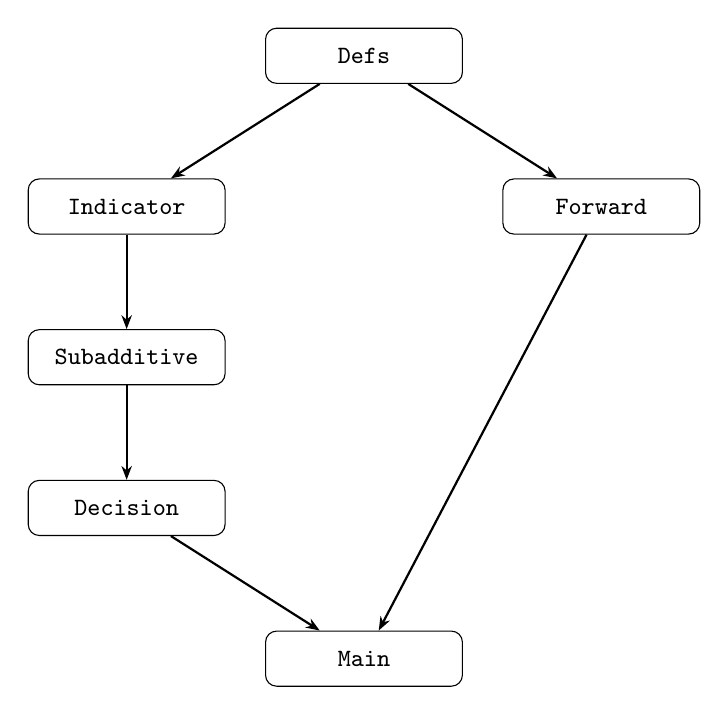
\begin{tikzpicture}[
  node distance=1.5cm,
  box/.style={draw, rounded corners, minimum width=2.5cm,
    minimum height=0.7cm, font=\small\ttfamily},
  arr/.style={-{Stealth[length=5pt]}, thick}
]
  \node[box] (defs) {Defs};
  \node[box, below left=1.2cm and 0.5cm of defs] (ind) {Indicator};
  \node[box, below right=1.2cm and 0.5cm of defs] (fwd) {Forward};
  \node[box, below=1.2cm of ind] (sub) {Subadditive};
  \node[box, below=1.2cm of sub] (dec) {Decision};
  \node[box, below right=1.2cm and 0.5cm of dec] (main) {Main};

  \draw[arr] (defs) -- (ind);
  \draw[arr] (defs) -- (fwd);
  \draw[arr] (ind) -- (sub);
  \draw[arr] (sub) -- (dec);
  \draw[arr] (dec) -- (main);
  \draw[arr] (fwd) -- (main);
\end{tikzpicture}
\end{center}

\subsection{Line Counts}

\begin{center}
\begin{tabular}{@{}llr@{}}
\toprule
\textbf{File} & \textbf{Content} & \textbf{Lines} \\
\midrule
\texttt{Defs.lean} & Core definitions (LPO, BMC, FeketeConvergence, encoding) & 87 \\
\texttt{Indicator.lean} & hasTrue/indicator properties (monotonicity, witnesses) & 118 \\
\texttt{Subadditive.lean} & Subadditivity and lower bound proofs & 103 \\
\texttt{Decision.lean} & Main theorem: $\FekConv \to \LPO$ & 117 \\
\texttt{Forward.lean} & Axiomatized forward direction & 43 \\
\texttt{Main.lean} & Assembly, equivalence theorem, axiom audit & 81 \\
\midrule
\textbf{Total} & & \textbf{549} \\
\bottomrule
\end{tabular}
\end{center}

\subsection{Key Design Decisions}

\begin{enumerate}[nosep]
\item \textbf{Bool encoding.} The binary sequence $\alpha$ is typed as
  $\NN \to \mathrm{Bool}$ (not $\NN \to \{0,1\} \subset \NN$). This
  makes case splits definitionally decidable without any lemma.

\item \textbf{Decidable bounded search via \texttt{List.any}.} The
  indicator uses \texttt{(List.range n).any} to compute $x_n$. This
  is computable and avoids any classical content in the encoding.

\item \textbf{Noncomputable section.} The \texttt{indicator} and
  \texttt{mockFreeEnergy} are marked \texttt{noncomputable} because
  they produce \texttt{Real} values (Mathlib's $\RR$ is
  noncomputable). The \emph{decision} (left/right disjunct of $\LPO$)
  is computed from Bool operations, not from the real-valued functions.

\item \textbf{Monotonicity does the work.} The subadditivity proof
  requires only that the indicator is monotone---no case split on
  Bool is needed. This yields a clean \texttt{nlinarith} proof.
\end{enumerate}

% ====================================================================
\section{Reproducibility}\label{sec:repro}
% ====================================================================

\begin{mdframed}[linecolor=black, linewidth=0.5pt,
  backgroundcolor=lean-bg, innertopmargin=8pt,
  innerbottommargin=8pt]
\textbf{Reproducibility box.}
\begin{center}
\begin{tabular}{@{}ll@{}}
\toprule
\textbf{Component} & \textbf{Version / Commit} \\
\midrule
Lean 4 & \texttt{v4.28.0-rc1} \\
Mathlib4 & \texttt{2598404fe9e0a5aee87ffca4ff83e2d01b23b024} \\
\bottomrule
\end{tabular}
\end{center}

\medskip\noindent
\textbf{Build instructions:}
\begin{verbatim}
  lake exe cache get     # download prebuilt Mathlib (~5 min)
  lake build             # compile Paper 29 (~2-5 min)
\end{verbatim}

\medskip\noindent
\textbf{Verification:} A successful build produces 0 errors, 0
warnings, 0 \texttt{sorry}s. The axiom audits in \texttt{Main.lean}
confirm the axiom profiles reported in~\S\ref{sec:audit}.

\medskip\noindent
All dependency versions are pinned in \texttt{lake-manifest.json}
for exact reproducibility.
\end{mdframed}

% ====================================================================
\section{Discussion}\label{sec:discussion}
% ====================================================================

\subsection{Resolution of Paper 10, Problem 1}\label{sec:resolution}

The main consequence of $\FekConv \leftrightarrow \LPO$ is a
resolution of Problem~1 from Paper~10~\cite{Lee26P10}: the $\LPO$
cost of the thermodynamic limit is ineliminable \emph{at the level
of Fekete's lemma}---the generic tool used for arbitrary interacting
systems. This yields a three-tier hierarchy for thermodynamic-limit
convergence:

\begin{center}
\begin{tabular}{@{}lll@{}}
\toprule
\textbf{Route} & \textbf{Logical cost} & \textbf{Example} \\
\midrule
Exact solution (closed-form modulus) & $\BISH$ &
  1D Ising (Papers~8, 9) \\
Cluster expansion (exponential decay) & $\BISH$ &
  High-$T$ lattice gases \\
Generic subadditivity (Fekete) & $\LPO$ &
  This paper \\
\bottomrule
\end{tabular}
\end{center}

\noindent
The first two tiers provide constructive convergence by exhibiting
explicit Cauchy moduli. The third tier---Fekete's lemma---extracts
convergence from a non-constructive infimum, and this extraction is
unavoidably $\LPO$.

\subsection{Physical Interpretation}\label{sec:physical}

The three-tier hierarchy has a natural physical interpretation.

\textbf{Tier 1 (exact solvability):} Systems like the 1D Ising chain
have closed-form partition functions (via transfer matrices, Bethe
ansatz, etc.) that yield explicit error bounds. The convergence rate
is typically exponential in the system size, with the rate depending
on the spectral gap of the transfer matrix. No omniscience is needed.

\textbf{Tier 2 (cluster expansions):} For high-temperature or
low-density systems, the cluster expansion~\cite{BF76,KP86} provides
an explicit convergent series for $\log Z_\Lambda$. The convergence
is controlled by a fugacity parameter or inverse temperature and
provides explicit moduli. The expansion converges when the activity
is below a critical threshold---precisely the regime where
correlations decay exponentially.

\textbf{Tier 3 (generic Fekete):} When neither exact solutions nor
convergent expansions are available---typically near phase transitions
where the correlation length diverges---the only route to the
thermodynamic limit is the generic subadditivity argument. Our result
shows this route costs exactly $\LPO$.

The physical picture is suggestive: $\LPO$ becomes necessary precisely
when the system loses its explicit finite-range structure. Phase
transitions, where correlations become long-range and cluster
expansions diverge, are the physical locus where the $\LPO$ cost
becomes ineliminable.

\subsection{Implications for Paper 10}\label{sec:paper10}

Paper~10~\cite{Lee26P10} articulated the ``logical geography
hypothesis'': each physical idealization occupies a specific position
in the constructive hierarchy. The present result prompted a
refinement of Paper~10's thesis (now incorporated in Paper~10 v5.0).

Paper~10's original formulation stated that the thermodynamic limit
costs $\LPO$. This is correct for the \emph{generic} route through
Fekete's lemma, but not for specific models with explicit solutions.
The refined thesis is:

\begin{quote}
\emph{The thermodynamic limit costs $\LPO$ via the generic
subadditivity route (Fekete's lemma). Exactly solvable models and
models within the convergence radius of cluster expansions bypass
Fekete and achieve convergence in $\BISH$. The $\LPO$ cost becomes
ineliminable at or near phase transitions.}
\end{quote}

\noindent
Paper~10 (v5.0) has been revised to incorporate this refinement,
with its calibration table (Table~1) now distinguishing between
the generic route ($\equiv \LPO$) and the model-specific routes
($\BISH$).

\subsection{The Boche--Bock--Deppe Connection}\label{sec:bbd}

Boche, Bock, and Deppe~\cite{BBD20} proved that the Fekete limit, as
a functional from subadditive sequences to $\RR$, is not
Banach--Mazur computable---it lies above the arithmetical hierarchy.
Our result shows a related but distinct fact: extracting the
\emph{existence} of the limit (not computing its value) already
requires $\LPO$.

Non-computability (a statement about Turing machines) and
non-constructivity (a statement about proof principles) are different
concepts, but they point in the same direction: the Fekete limit
resists effective extraction at multiple levels of the mathematical
hierarchy.

\subsection{Open Questions}\label{sec:open}

\begin{enumerate}
\item \textbf{Multi-dimensional subadditivity.} For $d > 1$, the
  subadditivity argument requires careful treatment of boundary
  effects (van Hove limits). Does the multi-dimensional version
  have the same $\LPO$ cost?

\item \textbf{Pressure functionals.} The thermodynamic formalism
  defines pressure as a supremum over measures. What is the
  constructive cost of this variational principle?

\item \textbf{Superadditivity.} Fekete's lemma applies equally to
  superadditive sequences ($u_{m+n} \geq u_m + u_n$). Is the
  $\LPO$ equivalence symmetric, or does one direction admit a
  weaker principle?

\item \textbf{Quantitative calibration.} Can the encoding be
  refined to give quantitative information about the relationship
  between the convergence rate of $u_n/n$ and the decidability
  speed of the binary sequence?
\end{enumerate}

% ====================================================================
\section{AI-Assisted Methodology}\label{sec:ai}
% ====================================================================

The encoding $F_n = -n \cdot x_n$ and the proof strategy for
$\FekConv \to \LPO$ were proposed by Gemini~3.0 DeepThink (Google
DeepMind) in response to a detailed prompt about the constructive
status of Fekete's lemma. The formalization in \Lean{}, including all
tactic proofs, was carried out by Claude (Anthropic). The author
supervised both stages, verified the mathematical content, and wrote
the paper.

This workflow---mathematical insight from one AI system, formalization
by another, supervision by a human---proved effective for bridging
the gap between conceptual mathematics and machine-checked proof.

% ====================================================================
% References
% ====================================================================
\begin{thebibliography}{99}

\bibitem{BBD20}
H.~Boche, Y.~Bock, and C.~Deppe.
\newblock On the computability of Fekete's subadditive lemma and
  applications.
\newblock \emph{IEEE Trans.\ Signal Process.}, 68:6757--6769, 2020.

\bibitem{BF76}
D.~Brydges and P.~Federbush.
\newblock A new form of the Mayer expansion in classical statistical
  mechanics.
\newblock \emph{J.\ Math.\ Phys.}, 17(12):2100--2107, 1976.

\bibitem{BV06}
D.~Bridges and L.~V\^{\i}\c{t}\u{a}.
\newblock \emph{Techniques of Constructive Analysis}.
\newblock Springer, 2006.

\bibitem{Fek23}
M.~Fekete.
\newblock \"Uber die {V}erteilung der {W}urzeln bei gewissen
  algebraischen {G}leichungen mit ganzzahligen {K}oeffizienten.
\newblock \emph{Math.\ Z.}, 17(1):228--249, 1923.

\bibitem{FV17}
S.~Friedli and Y.~Velenik.
\newblock \emph{Statistical Mechanics of Lattice Systems: A Concrete
  Mathematical Introduction}.
\newblock Cambridge University Press, 2017.

\bibitem{Ish06}
H.~Ishihara.
\newblock Reverse mathematics in {B}ishop's constructive mathematics.
\newblock \emph{Philosophia Scientiae, Cahier Sp\'ecial},
  6:43--59, 2006.

\bibitem{KP86}
R.~Koteck\'y and D.~Preiss.
\newblock Cluster expansion for abstract polymer models.
\newblock \emph{Comm.\ Math.\ Phys.}, 103(3):491--498, 1986.

\bibitem{Lee26P8}
P.~C.-K.~Lee.
\newblock The logical cost of the thermodynamic limit:
  {LPO}-equivalence and {BISH}-dispensability for the {1D} {I}sing
  free energy.
\newblock Preprint, 2026.
\newblock \Lean{} formalization.

\bibitem{Lee26P9}
P.~C.-K.~Lee.
\newblock Combinatorial {I}sing encoding for {BMC}$\to${LPO}.
\newblock Preprint, 2026.
\newblock \Lean{} formalization (Paper~9).

\bibitem{Lee26P10}
P.~C.-K.~Lee.
\newblock Logical geography of mathematical physics: a constructive
  calibration programme.
\newblock Preprint, 2026.
\newblock Paper~10 (synthesis).

\bibitem{Mathlib}
The Mathlib Community.
\newblock \emph{Mathlib4}.
\newblock \url{https://github.com/leanprover-community/mathlib4},
  2024--2026.

\bibitem{Rue69}
D.~Ruelle.
\newblock \emph{Statistical Mechanics: Rigorous Results}.
\newblock W.\,A.\ Benjamin, New York, 1969.

\bibitem{vW19}
T.~van Wierst.
\newblock Constructive analysis in the {A}gda proof assistant.
\newblock MSc thesis, University of Amsterdam, 2019.

\end{thebibliography}

\end{document}
